\section{Mapping Instructions and Visual Observations to Actions}
In ~\cite{DBLP:journals/corr/MisraLA17}, they propose to directly map raw visual observations and text input to actions for instruction execution.  While existing approaches assume access to structured environment representations or use a pipeline of separately trained models, they learn a single model to jointly reason about linguistic and visual input. They use reinforcement learning in a contextual bandit setting to train a neural network agent. To guide the agent’s exploration, they use reward shaping with different forms of supervision.

\begin{figure}[htbp]
    \centering
    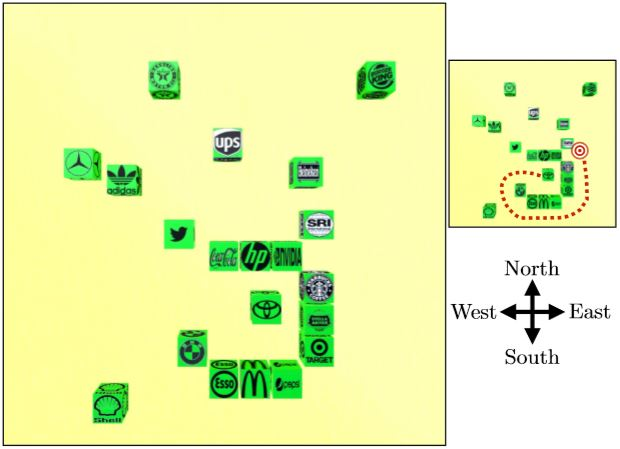
\includegraphics[width=.8\textwidth]{block}
    \caption{Blocks environment~\cite{DBLP:journals/corr/MisraLA17}}
\end{figure}
\newpage
\begin{table}[h!]
    \begin{tabular}{|p{15cm}|}
    \hline
    Put the Toyota block in the same row as the SRI block, in the first open space to the right of the SRI block.\\
    \hline
    Move Toyota to the immediate right of SRI, evenly aligned and slightly separated.\\
    \hline
    Move the Toyota block around the pile and place it just to the right of the SRI block.\\
    \hline
    Place Toyota block just to the right of The SRI Block.\\
    \hline
    Toyota, right side of SRI.\\
    \hline
    \end{tabular}
    \caption{Instructions in the Blocks environment~\cite{DBLP:journals/corr/MisraLA17}}
    \label{tab:1}
\end{table}

In Table~\ref{tab:1}, illustrates the matter within the Blocks surroundings. The agent observes the surroundings as RGB image employing a camera sensing element. Given the RGB input, the agent should acknowledge the blocks and their layout. To grasp the instruction, the agent should determine the block to maneuver (Toyota block) and also the destination (just right side of the SRI block). This needs determination linguistics and grounding issues. For instance, contemplate the top instruction within the figure. The agent has to determine the phrase pertaining to the block to maneuver, Toyota block, and ground it. It should resolve and ground the phrase SRI block as a reference position, that is then changed by the spatial which means recovered from a similar row as or initial open area to the correct of, to spot the goal position. Finally, the agent has to generate actions, for instance moving the Toyota block around obstructing blocks.

To address these challenges with one model, they create a neural network agent. The agent executes directions by generating a sequence of actions. At every step, the agent takes as input the instruction text, observes the planet as RGB image, and selects consequent actions. Action execution changes the state of the environment. Given observation of the new environment state, the agent selects consequent action. This method continues till the agent indicates execution completion. Once choosing actions, the agent together reasons concerning its observations and also the instruction text. This permits selections supported shut interaction between observations and linguistic input.

They study the problem of learning to execute instructions in a situated environment given only raw visual observations. Supervised approaches do not explore adequately to handle test time errors, and reinforcement learning approaches require a large number of samples for good convergence. Their solution provides an effective combination of both approaches: reward shaping to create relatively stable optimization in a contextual bandit setting.

This combination is designed for a few-samples regime, as we address. When the number of samples is unbounded, the drawbacks observed in this scenario for optimizing longer term reward do not hold.
